\documentclass[10pt,twocolumn,letterpaper]{article}

\usepackage{cvpr}
\usepackage{times}
\usepackage{epsfig}
\usepackage{graphicx}
\graphicspath{{/home/li/图片/}}
\usepackage{amsmath}
\usepackage{amssymb}
\usepackage{fontspec}

\usepackage[pagebackref=true,breaklinks=true,letterpaper=true,colorlinks,bookmarks=false]{hyperref}

\cvprfinalcopy % *** Uncomment this line for the final submission

\def\cvprPaperID{****} % *** Enter the CVPR Paper ID here
\def\httilde{\mbox{\tt\raisebox{-.5ex}{\symbol{126}}}}

\ifcvprfinal\pagestyle{empty}\fi
\setcounter{page}{1}

\begin{document}

\author{Qingyun Li\\\\
July 12, 2018}        
\title{GAN}

\maketitle

\section{Tntroduction}
\par The  framework can yield specific training algorithms for many kinds of model and optimization algorithm. In the article, the authors explore the special case when the generative model generates samples by passing random noise through a multilayer perceptron, and this discriminative model is also a multilayer perceptron. We refer to this special case as adversarial nets. In this case, we can train both models and using only the highly successful backpropagation and dropout algorithms~\cite{Hinton2012Improving} and sample from the generative model using only forward propagation. No approximate inference or Markov chains are necessary.
\section{Related work}
\par An alternative to directed graphicalmodels with latent variables are undirected graphical models with latent variables, such as restricted Boltzmann machines (RBMs)~\cite{smolensky1986information}, deep Boltzman machines (DBMs)~\cite{salakhutdinov2010efficient} and their numerous variants. The interactions within such models are represented as the product of unnormalized potential functions, normalized by a global summation over all states of the random variables. This quantity and its gradient are intracble for all but the most trivial instances, although they can be estimated by Markov chain Monte Carlo (MCMC) methods\footnote{A Markov chanin is a stochastic model describing a sequence of possible events in which the probability of each event depends only on the state attained in the previous event. Roughly speaking, a process satisfies the Markov property if one can make predictions for the future based only on its present state just as well as one could knowing the process's full history. In statistics, MCMC methods comprise a class of algorithms for sampling from a probability distribution. By constructing a Markov chain that has the desired distribution as its equilibrium distribution, one can obtain a sample of the desired distribution by observing the chain after a number of steps. The more steps there are, the more closely the distribution of the sample matches the actual desired distribution.}. Mixing poses a significant problem for learning algorithms that rely on MCMC~\cite{bengio2013better}.
\par Deep belief networks (DBNs) are hybrid models containing a single undirected layer and several directed layers. While a fast approximate layer-wise training criterion exists, DBNs incur the computational difficulties associated with both undirected and directed models.
\par Alternative criteria that do not approximate or bound the log-likelihood have also been proposed, such as score matching~\cite{Hyv2005Estimation} and noise-contrasive estimation (NCE)~\cite{Gutmann2010Noise}. Both of these require the learned probability density to be analytically specified up to a normalization to be analytically specified up to a normalization constant. Note that in many interesting generative models with several layers of latent variable (such as DBNs and DBMs), it is not even possible to derive a tractable unnormalized probability density. Some models such as denoising auto-encodes~\cite{Vincent2008Extracting} and contractive autoencoders have learning rules very similar to score matching applied to RBMs. In NCE, as in this work, a discriminative training criterion is employed to fit a generative model. However, rather than fitting a separate discriminative model, the generative model itself  is used to discriminate generated data from samples a fixed noise distribution. Because NCE uses a fixed noise distribution, learning slows dramatically after the model has learned even an approximately correct distribution over a small subset of the observed variables. 
\par Finally, some techniques do not involve defining a probability distribution explicitly, but rather train a generative machine to draw samples from the desired distribution. This approach has the advantage that such machines can be designed to be trained by back-propagation. Prominent recent work in this area includes the generative stochastic network (GSN) framework~\cite{Bengio2014Deep}, which extends generalized denoising auto-encoders~\cite{Bengio2013Generalized}: both can be seen as defining a parameterized Markov chain. Compared to GSNs, the adversarial nets framework does not require a Markov chain for sampling. Because adversarial nets do not require feedback loops during generation, they are better able to leverage piecewise linear units~\cite{Jarrett2010What}, which improve the performance of backpropagation but have problems with unbounded activation when used ina feedback loop. More recent examples of training a generative machine by back-propagation into it include recent work on auto-encoding variational Bayes and stochastic backpropagation.
\section{Adversarial nets}
\par The adversarial modeling framework is most straightforward to apply when the models are both multilayer perceptions. To learn the generator's distribution $p_{g}$ over data x, we define a prior on input noise variable $p_{z}(z)$, then represent a mapping to data space as $G(z;\theta_{g})$,where G is a differentiable function represented by a multilayer perceptron with parameters $\theta_{g}$. We also define a second multilayer perceptron $D(x;\theta_{d})$ that outputs a single scalar. D(x) represents the probability that x came from the data rather than $p_{g}$. We train D to maximize the probability of assigning the correct label to both training examples and samples from G.
\par The authors make a theoretical analysis of adversarial nets, essentially showing that the training criterion allows one to recover the data generating distribution as G and D are given enough capacity, i.e.\ in the non-parameter limit. See Figure.~\ref{GAN} for a less formal, more pedagogical explanation of the approach. In practice, we must implement the game using an iterative, numerical approach. Optimizing D to completion in the inner loop of training is computationally prohibitive, and on finite datasets would result in overfitting. I stead, we alternate between k steps of optimizing D and one step of optimizing G. This results in D being maintained near its optimal solution, so long as G changes slowly enough. This strategy is analogous to the way that SML/PCD~\cite{younes1999convergence} training maintains samples from a Markov chain from one learning step to the next in order to avoid burning in a Markov chain as part of the inner loop of learning.
\begin{figure}[htbp]
 \centering{}
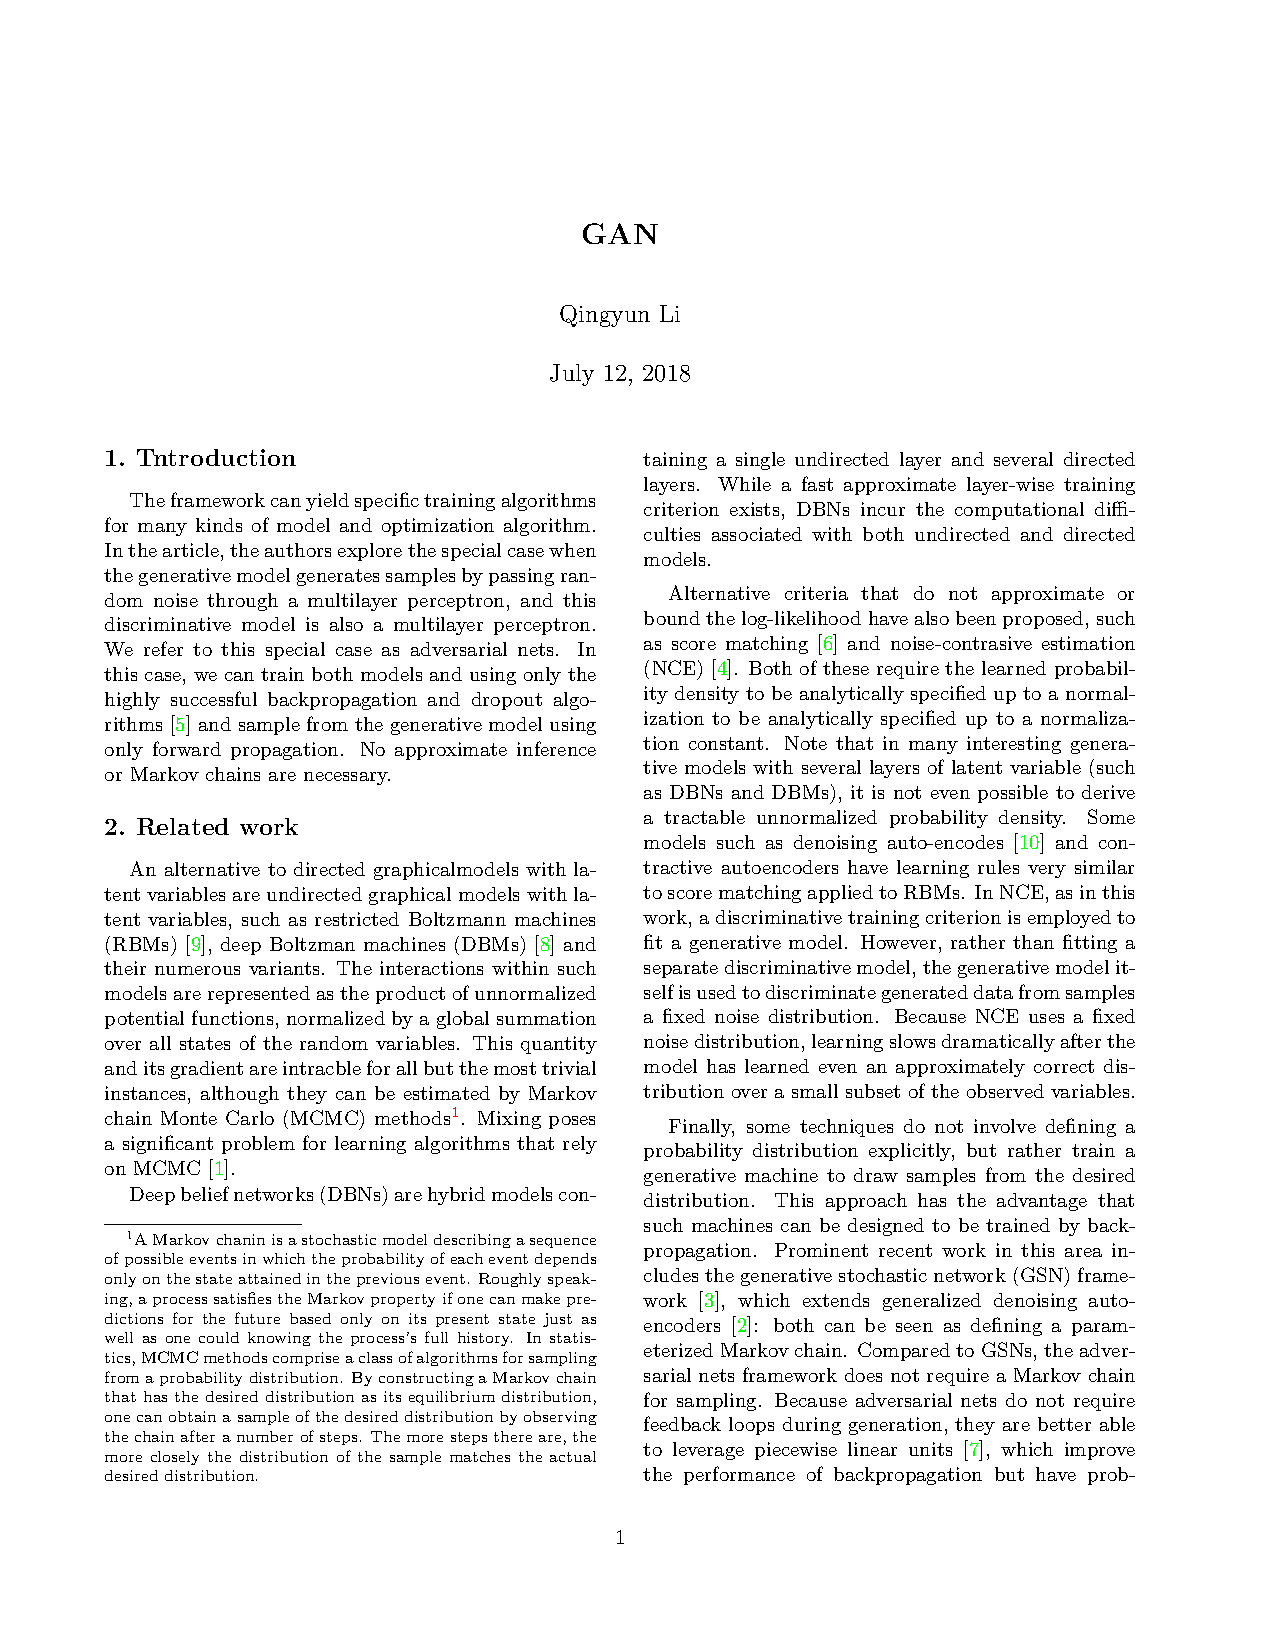
\includegraphics[width=0.7\linewidth]{GAN.png}\\
 \caption{Procedure of training.}
\label{GAN}
\end{figure}
  \bibliographystyle{ieee}
 \bibliography{single}
\end{document}
